% Supplementary Material for
%   "Validation protocol reverses machine-learning model rankings in tokamak
%    energy-confinement scaling"
%
% Build:  tectonic paper/supplementary.tex
%
% This file is a standalone document with its own reference list, as IOP asks
% of supplementary files. Every number in it is regenerated by the same scripts
% as the main text; see the repository named in the main paper.
\documentclass[12pt,a4paper]{article}

\usepackage[margin=2.4cm]{geometry}
\usepackage[T1]{fontenc}
\usepackage{lmodern}
\usepackage{amsmath}
\usepackage{booktabs}
\usepackage{graphicx}
\graphicspath{{../results/}{./}}
\DeclareGraphicsExtensions{.pdf,.png}
\usepackage{caption}
\usepackage{microtype}
\usepackage[hidelinks]{hyperref}
% Switched on by `make review-pdf` for the review upload only; see paper.tex.
% \usepackage[mathlines]{lineno}\linenumbers
\usepackage{xcolor}
\usepackage{siunitx}
\usepackage[section]{placeins}

\captionsetup{font=small,labelfont=bf}
\setlength{\parskip}{0pt}
\sisetup{detect-all}
% Long \texttt{} identifiers (scikit-learn class names) are single unbreakable
% words wider than the slack a 12 pt line normally carries. Rather than
% hyphenating a code identifier, which would be wrong to copy out, let TeX
% distribute the shortfall across the paragraph.
\setlength{\emergencystretch}{3em}

\renewcommand{\thesection}{S\arabic{section}}
\renewcommand{\thetable}{S\arabic{table}}
\renewcommand{\thefigure}{S\arabic{figure}}

% IOP asks each supplementary file for a title of at most 30 characters and a
% description of at most 30 words. Those are the two lines directly below; the
% article title follows underneath, where it orients a reader without being
% mistaken for the formal supplementary title.
\title{\vspace{-1.4cm}\textbf{Supplementary material}}
\author{Liam Salcedo\thanks{Independent researcher, Montclair, New Jersey, USA.
\texttt{liamsalcedo100@gmail.com}.
ORCID: \href{https://orcid.org/0009-0001-5039-8147}{\texttt{0009-0001-5039-8147}}.}}
\date{8 September 2026}

\begin{document}
\maketitle

\begin{center}\small
\textbf{Description.} Supporting analyses for the main text: interval
recalibration, rows outside the standard analysis set, a locked device forecast,
and two replications on allometric scaling laws outside fusion.
\end{center}

\vspace{0.4em}
\noindent\textbf{For:} ``Validation protocol reverses machine-learning model
rankings in tokamak energy-confinement scaling'' (L. Salcedo).

\vspace{0.6em}
\noindent This document holds the supporting analyses referred to in the main
text. Sections~S1 to~S3 are fusion analyses whose headline numbers are stated in
the main text and whose construction, tables and caveats are given here in full:
repairing the interval collapse and finding the limit of the repair, replicating
the ranking inversion on rows the standard analysis set excludes, and a locked
forecast at three device operating points. Sections~S4 and~S5 are the two
replications outside fusion. Sections~S6 to~S8 are supporting material for
results the main text states in prose: the three-kernel Gaussian-process ladder
behind the mean-function ablation, the full model, kernel and split
specification, and the per-label scores with the eligibility-threshold sweep.
Sections~S9 and~S10 are two results the main text summarises in a paragraph
each: a power law with a bounded correction, and the mixed model the
clustered-validation literature pairs with this split design.

Why those two belong in a fusion paper is argued where they are first
introduced, in the Discussion of the main text: HDB5 cannot separate the
extrapolation failure from the ranking inversion, because on its nine features
the flexible model always wins the interpolation split, and the nested predictor
ladder of Sec.~\ref{sec:ladder} can. Neither replication is evidence the
confinement result depends on.

Section and equation numbers prefixed S refer to this document; unprefixed
section names refer to the main text.

Each section here is a result the main text states and relies on. What moved is
the construction, the tables and the caveats, not the finding.

\section{Repairing the intervals, and the limit of the repair}
\label{supp:shift}

The diagnosis in the calibrated-intervals section of the main text makes a testable prediction. If the interval collapse
is really about exchangeability rather than about the models, then calibrating
on held-out \emph{labels} instead of held-out discharges should repair it, and
should repair it only as far as that unit reaches. Both halves are tested below.

The label-level scheme uses an inner leave-one-label-out loop, and nothing in
it touches the target label. It is called label-level rather than machine-level
deliberately: the calibration unit is the database device/wall label, so for a
target of JET-ILW the calibration set still contains JET. The device-level
variant that removes that overlap is reported at the end of this section. For
each target $m$: remove $m$; the remaining labels are the training set. Inside
that training set, hold out each label $k$ with at least 30 rows in turn, fit on the others, and record
$\lvert \log\hat\tau - \log\tau \rvert$ on $k$ together with each of its rows'
Mahalanobis distance from that inner fit set. Pool those residuals into the
calibration quantile. Then fit the final model on all the training labels and
score $m$ once. Every conformity score therefore comes from a label its own
model had not seen, which is the unit the test rows differ by, and no row from
$m$ enters any fit or any quantile. The distance-scaled variant fits
$\sigma(d)=\exp(c_0 + c_1 d)$ to those calibration residuals by least squares on
$\log\lvert r \rvert$ and divides the scores by it.

Neither scheme is a finite-sample-valid group-conformal procedure, and they are
not claimed as one. Two things stand in the way. The conformity score is still a
row, not a label, and rows arrive in correlated clusters, so the exchangeability
the split-conformal proof needs is no more available here than in
the calibrated-intervals section of the main text. And in the distance-scaled arm the scale function
$\sigma(d)$ is estimated from the same calibration residuals it then normalises,
which the standard argument does not cover. What these are is empirical
held-out-label residual calibration: the quantile is the finite-sample
conformal rank applied to those scores, and the coverage reported for it is
measured rather than guaranteed. Recovering a guarantee would need
label-level conformity scores and a scale model fitted on separate rows or
cross-fitted, and neither is done here.

\begin{table}[t]
\centering
\small
\caption{Empirical coverage of nominal 90\% intervals under three calibration
schemes, on a held-out database label (LOLO) and across the ITER-size-matched
cut. The device-level counterpart is Table~\ref{tab:supdevice}.}
\label{tab:supshift}
\begin{tabular}{lrrrrrr}
\toprule
& \multicolumn{2}{c}{split conformal} & \multicolumn{2}{c}{by label}
& \multicolumn{2}{c}{$+$ distance} \\
\cmidrule(lr){2-3}\cmidrule(lr){4-5}\cmidrule(lr){6-7}
Model & LOLO & cut & LOLO & cut & LOLO & cut \\
\midrule
random forest & 35\% & 3\% & \textbf{88\%} & 29\% & 88\% & 40\% \\
hist grad.\ boosting & 45\% & 0\% & \textbf{90\%} & 4\% & 89\% & 13\% \\
ridge, log-linear & 83\% & 70\% & 91\% & 77\% & 92\% & 82\% \\
power law, collisionless & 85\% & 91\% & 91\% & \textbf{95\%} & 92\% & 92\% \\
IPB98(y,2)$^{*}$ & 89\% & 88\% & 89\% & 89\% & 89\% & 87\% \\
\bottomrule
\end{tabular}
\end{table}

Both arms behave as the diagnosis predicts. On a held-out label, empirical
row-level coverage returns close to nominal: every model lands within two points
of it, tree ensembles included, and the random forest goes from 35\% to 88\%.
Across the size cut none does. Neither recalibration procedure tested restores
near-nominal coverage there, because every calibration unit is smaller than
every test unit, and scaling the interval by extrapolation distance recovers
only part of the gap (3\% to 40\% for the forest).

\paragraph{The same calibration over physical devices.} The scheme above
calibrates on database labels, so for a target of JET-ILW the calibration set
still contains JET. Collapsing the wall variants and repeating the whole
procedure over the 11 physical devices removes that overlap: training,
calibration and scoring then all use the device as the unit.

\begin{table}[!htbp]
\centering
\small
\caption{The same three schemes with wall variants collapsed, so every
calibration unit is a physical device and the held-out device is genuinely
unseen. Pooled row-level coverage of nominal 90\% intervals, with the median
multiplicative half-width in brackets.}
\label{tab:supdevice}
\begin{tabular}{lrrr}
\toprule
Model & split conformal & by device & $+$ distance \\
\midrule
random forest            & 31\% (1.23$\times$) & 84\% (2.46$\times$) & 88\% (2.76$\times$) \\
hist grad.\ boosting     & 38\% (1.24$\times$) & 77\% (2.29$\times$) & 80\% (2.53$\times$) \\
ridge, log-linear        & 85\% (1.34$\times$) & 92\% (1.40$\times$) & 93\% (1.43$\times$) \\
power law, collisionless & 88\% (1.34$\times$) & 92\% (1.39$\times$) & 93\% (1.42$\times$) \\
IPB98(y,2)$^{*}$         & 90\% (1.39$\times$) & 90\% (1.39$\times$) & 90\% (1.39$\times$) \\
\bottomrule
\end{tabular}
\\[2pt]
{\footnotesize $^{*}$historical reference, not refitted within these folds.}
\end{table}

Table~\ref{tab:supdevice} says the diagnosis holds and the repair is less complete
than the label-level numbers suggest. Plain split conformal is worse on a
genuinely unseen device than on an unseen label, 31\% against 35\% for the
forest and 38\% against 45\% for the booster, which is what removing the
within-device overlap should do. Calibrating by device then recovers most of
the shortfall for the forest (84\%, and 88\% with distance scaling, against
88\% either way at label level) but noticeably less for the booster, which
reaches 77\% and 80\% where the label-level scheme reported 90\% and 89\%. The
label-level number therefore overstates how well this repair calibrates the
booster on a device it has never seen. Both linear models are unaffected within
a point or two. The cost is visible in the widths: the trees buy that coverage
at roughly $2.3$ to $2.8\times$ multiplicative half-width against $1.23\times$
under plain split conformal, where the linear models stay near $1.4\times$.

Across the size cut with the same device grouping the picture is unchanged in
kind. The forest and booster remain far from nominal at 41\% and 12\% by device
and 57\% and 21\% with distance scaling, better than the label-level 29\% and
4\% but nowhere near 90\%, while the constrained power law holds at 95\% and
93\%. Changing the calibration unit cannot repair a shift the calibration set
does not contain, which is the point of the section.

Among the models refitted within folds, the constrained power law of
the constraint section of the main text is the only one in Table~\ref{tab:supshift} whose plain
split-conformal coverage stays near nominal at the ITER-size-matched cut, and its
intervals hold there under every scheme. IPB98(y,2) also holds at 88\%, but it
is a historical reference rather than a fold-fitted competitor.

\section{Robustness on rows the standard analysis set excludes}

Everything above rests on one file, which is a central limitation of the preceding analysis.
The same OSF project publishes the full database revision, DB5.2.3, with 14153
rows against STD5's 6228, and it is pinned by its own SHA-256. Matching on
(tokamak, shot, time) shows STD5 is an ELMy-H-mode quality selection out of it
and leaves two populations this study had not analysed: \textbf{5358 H-mode rows
STD5 does not contain} (12 labels, zero row overlap) and \textbf{3860 ohmic
and L-mode rows} in a different confinement regime, scored against
ITER89-P~\cite{iter89p} because an H-mode law is the wrong baseline for an
L-mode plasma.

This replication has one failure mode that would not announce itself. If the
row match against STD5 fails, every STD5 row stays in the ``disjoint'' arm, that
arm becomes a superset of the data the ranking-inversion section of the main text was computed on, and
it reproduces the ranking-inversion section of the main text by construction. The matcher is therefore
checked positively as well as negatively: STD5 matched against itself must
overlap completely, and the disjoint arm must share zero rows.

The ranking inverts in both arms. On the disjoint H-mode rows the best
cross-validated model beats the published law by 42\%, a margin of the same
size as the 36\% over that law reported above and computed on rows it never
saw, and the best model on an unseen label is IPB98(y,2). On the ohmic and L-mode rows the
cross-validation gain over ITER89-P is 67\% and the best model on an unseen
label is the collisionless power law of the constraint section of the main text. Counting label--model pairs
where a tree ensemble loses to the published law on an unseen label: 19 of 24
and 10 of 10.

Row disjointness is not discharge disjointness, and the paper's own argument
says the discharge is the unit that matters. Of the 5358 H-mode rows, 425
(7.9\%) are slices of one of 336 discharges that STD5 samples at a different
time. Dropping those discharges outright leaves 4933 rows across 2864
discharges that share no shot with STD5 at all, and the arm survives: the best
cross-validated model still beats the published law, by 39\% against 41\% on the
full arm, and the best model on an unseen label is still IPB98(y,2), with the
tree ensembles at 0.526 and 0.552 against the power law's 0.332. The reversal
does not depend on the shared discharges.

So the reversal is not an artefact of the standard set's selection criteria, and
not a property of ELMy H-mode or of IPB98(y,2) specifically. It is emphatically
\emph{not} an independent database: both arms come from the same ITPA collection
and the same devices, and the five-machine arm is too small to carry a claim
alone.

\section{Locked predictions at three device operating points without matching
H-mode observations}

Everything above is retrospective. To make the disagreement checkable rather
than merely described, what each model predicts is recorded for three real
devices, with intervals, a date, and a digest over the input rows so that a
later edit is visible. The parameter sets are published design values, and
for SPARC and ITER, evaluating IPB98(y,2) on the adopted design vector
reproduces the reference confinement time its own source quotes, to 0.6\% and
2.9\% respectively; the JT-60SA source supplies operating parameters rather than
a quoted confinement time. Those are checks that the right machine is being
described. None of the three has a \emph{measured} H-mode thermal confinement
time at the operating point tabulated here, which is what makes these
predictions rather than retrodictions.

The ITER row is taken from the 1999 basis~\cite{ipb98}, and a forecast whose
whole purpose is to be checkable later should say why it is locked against a
document of that age. The eight engineering values it supplies for the $Q=10$
inductive scenario, $R=\SI{6.2}{\metre}$, $a=\SI{2.0}{\metre}$,
$I_p=\SI{15}{\mega\ampere}$, $B_t=\SI{5.3}{\tesla}$,
$\bar{n}_e=\SI{10e19}{\per\cubic\metre}$, $P=\SI{87}{\mega\watt}$,
$\kappa=1.7$ and $M=2.5$, are the ones the 2007 revision of the confinement and
transport basis carries forward for the same scenario~\cite{doyle07}, so the
choice is not a 1999 number that a 2007 number would replace. ITER's programme
has been rebaselined since, on a schedule and a staging this paper does not
attempt to summarise and cites nothing for, so the row should be read as
conditional on the operating point tabulated above rather than on ITER's current
plan of record. It is not a prediction of whatever ITER's first $Q=10$ discharge
turns out to be, and a reader who prefers a different operating point can
rescore every model at one: the complete input vector is in
\texttt{results/forecast.json}.

\begin{table}[!ht]
\centering
\small
\caption{Predicted energy confinement time, in seconds, with nominal 90\%
intervals. Locked 31 August 2026 against a fixed dataset digest, so that the operating
points these were computed at can be recovered later. Operating
points are published design values: SPARC from~\cite{creely} (V2 primary
reference discharge), ITER from~\cite{ipb98} ($Q=10$ inductive baseline), and
JT-60SA from its Research Plan~\cite{jt60saplan} (full-current inductive
scenario). Intervals are distance-scaled held-out-label calibration intervals, not
the plain split-conformal intervals of the main text's coverage table, and are
pointwise intervals for a new observation; their construction is specified in
the text below. The complete input vector for each device is recorded in
\texttt{results/forecast.json} under the content digest quoted below.}
\label{tab:supforecast}
\begin{tabular}{lccc}
\toprule
& SPARC & JT-60SA & ITER \\
& \SI{1.85}{\metre} & \SI{2.96}{\metre} (operating) & \SI{6.2}{\metre} \\
\midrule
IPB98(y,2)$^{*}$ & 0.765 [0.58, 1.00] & 0.479 [0.35, 0.66] & \textbf{3.591 [2.66, 4.85]} \\
power law, collisionless & 0.724 [0.55, 0.96] & 0.428 [0.31, 0.59] & 2.837 [2.09, 3.84] \\
ridge, log-linear & 0.720 [0.53, 0.98] & 0.444 [0.32, 0.62] & 2.858 [2.07, 3.95] \\
random forest & 0.136 [0.03, 0.53] & 0.449 [0.23, 0.87] & \textbf{0.435 [0.19, 0.98]} \\
hist grad.\ boosting & 0.305 [0.14, 0.69] & 0.418 [0.24, 0.74] & 0.444 [0.24, 0.84] \\
\bottomrule
\end{tabular}
\end{table}

\paragraph{How these intervals are built.} They are not the plain
split-conformal intervals of the calibrated-intervals section of the main text, and deliberately so:
the main text's coverage table measures those covering 3\% of rows across the
ITER-size-matched cut, so quoting them for a next-step device would publish an
interval already known to fail in exactly this situation. Each row instead uses
the distance-scaled label-level scheme of Sec.~\ref{supp:shift}, which gives the
best size-cut calibration for the models that fail most severely there, applied
with the whole
database as the training set. Two disclosures belong with that. The scheme was
chosen after comparing the three in Table~\ref{tab:supshift}, so these intervals
are exploratory rather than prospectively selected, in the same sense as the
constraint rung of the constraint section of the main text. And it calibrates over database
labels rather than physical devices, so these are not device-level conformal
intervals: Table~\ref{tab:supdevice} measures what that distinction costs, and for
the tree ensembles it is not negligible. The label-level scheme is retained here
because it is the one the forecast was locked under on 31 August 2026, and
re-deriving the intervals afterwards would make the lock meaningless. A reader
who prefers the device-level calibration should read the tree rows of
Table~\ref{tab:supforecast} as correspondingly optimistic in width. For a given model, each eligible label $k$ is
held out in turn, the model is refitted on the remaining labels, and the
absolute log residuals on $k$ are recorded together with each of its rows'
Mahalanobis distance $d$ from that inner fit set. A scale
$\sigma(d)=\exp(c_0+c_1 d)$ is fitted to those pairs by least squares on
$\log\lvert r\rvert$, dropping exactly-zero residuals; the conformity scores are
the residuals divided by $\sigma(d)$; and the half-width is the
$\lceil (n+1)(1-\alpha)\rceil$-th smallest such score at $\alpha=0.10$, the same
finite-sample rank used in the calibrated-intervals section of the main text. The interval reported for a
device is that quantile multiplied by $\sigma(d)$ evaluated at the device's own
distance, applied symmetrically in $\log\tau$ and exponentiated. The model whose
point prediction is tabulated is then fitted once on all 6228 rows. For
IPB98(y,2) the same construction is used on its analytic residuals, so its
interval is comparable to the others rather than merely coexisting with them.
Every interval is therefore an empirical pointwise calibration interval for a
new observation rather than a finite-sample-valid conformal interval. Three
things stand in the way, and only the last is about ITER: the conformity scores
remain clustered row-level scores, the distance scale is estimated from the
calibration residuals it normalises, and every calibration unit is smaller than
ITER along the size direction, which is the limitation
Sec.~\ref{supp:shift} measures directly.

Table~\ref{tab:supforecast} illustrates the practical consequence of the
disagreement in one place. On JT-60SA,
which sits inside the database's size range and is already operating, all five
models agree to within 15\%. On ITER, $1.82\times$ beyond it, they disagree by a
factor of \textbf{8.3}.

For the random forest that gap cannot be closed by tuning the standard
estimator, and the ranking-inversion section of the main text says why: it predicts by averaging
training targets, so its output cannot exceed the largest one, which here is
\SI{1.321}{\second}, and no hyperparameter moves that ceiling. The gradient
booster carries no corresponding arithmetic bound but produces a similarly low
point prediction. Because its prediction cannot exceed the largest training
target, \SI{1.321}{\second}, the random forest cannot reach the
\SIrange{2.84}{3.59}{\second} range the linear and physics-informed models
predict for this ITER operating point, and its nominal 90\% interval there runs
from \SI{0.19}{\second} to \SI{0.98}{\second}, containing none of those
predictions.

The JT-60SA column becomes checkable first, though not against any measurement
published as of the 31 August 2026 forecast lock: the first campaign ran L-mode
divertor plasmas, and its published power balance reports the energy confinement
time following L-mode scaling~\cite{jt60saop1}, whereas the row above is an
H-mode prediction scored against IPB98(y,2). Checking it needs H-mode operation
at a comparable design point, which the research plan~\cite{jt60saplan} places
in a later campaign and which the overview of first operation and forward
plans~\cite{jt60saop2} discusses in view of ITER and DEMO; no date is put on that here, because the
schedule is not ours to assert and the prediction is locked against a parameter
vector rather than against a calendar.

Each row of Table~\ref{tab:supforecast} carries its own interval and is assessed
separately against it, so the range quoted here names one model rather than the
set. A stationary JT-60SA H-mode near this design point reporting a thermal
confinement time outside \SIrange{0.349}{0.657}{\second} would fall outside the
IPB98(y,2) reference row's stated 90\% predictive interval. The fitted rows are
assessed at their own bounds, which are narrower for the constrained power law
(\SIrange{0.313}{0.587}{\second}) and wider for the random forest
(\SIrange{0.232}{0.867}{\second}). A single observation outside a nominal 90\%
interval is evidence against that forecast rather than a refutation of it: a
perfectly calibrated model still places about one observation in ten outside
such an interval, so a single miss is inconsistent with the prediction at the
stated interval level and no more. Because all five intervals overlap across
roughly this range, a measurement inside it separates none of them: this row
tests whether any model is right, not which, and that is why the ITER column
carries the argument.

Nothing above anticipated one feature of this table: SPARC sits further from
the training data than ITER does, at a Mahalanobis distance of 6.9 against 4.7,
despite being the smaller machine. Its \SI{12.2}{\tesla} field is 2.1 times the
largest toroidal field anywhere in the cleaned STD5 rows, \SI{5.82}{\tesla} on
Alcator C-Mod, and every other label in the database tops out at or below
\SI{4.80}{\tesla}. Size is not the only direction in which a next-step device
leaves the data behind, and an extrapolation audit organised around size alone
would have missed it.

\section{The same audit on a scaling law from another science}
\label{sec:allometry}

Every result in the main text rests on ITPA data, which leaves open whether any
of it is a fact about fusion specifically. Mammalian basal metabolic rate against body mass is
the same object and the older one: Kleiber~\cite{kleiber} found in 1932 that
metabolic rate scales as mass to the 3/4. Whether the true exponent is 3/4 or
2/3 has been argued for decades and this paper takes no position; 3/4 is used here as the
canonical historical reference law a fitted model has to beat. Taxonomic \emph{order} is the
unit a species belongs to, as a tokamak is the unit a discharge belongs to, and
\emph{body mass} is the axis a next instance lies beyond, as machine size is.
The data is Supplement 1 of a metabolic-rate compilation deposited on Figshare
(article 3549807), pinned by SHA-256 as the HDB5 files are, giving 541 species
records across 11 orders whose median masses span 342x. The analysis runs
through the domain-agnostic module released with this work rather than a copy
of the fusion pipeline, so it is the procedure a reader would apply to their
own data, and the problem has a \emph{single predictor}: no model can win by
finding a better combination of features, so the only thing separating them is
functional form. Refitting the exponent freely gives 0.687 against Kleiber's
0.75, so the constraint is not free here either.

\begin{table}[t]
\centering
\small
\caption{Kleiber's law under the same three splits. Scores are log-RMSE.}
\label{tab:allometry}
\begin{tabular}{lrrr}
\toprule
Model & CV, by species & leave-one-order-out & widest mass cut \\
\midrule
Kleiber, exponent 3/4 & 0.396 & 0.440 & \textbf{0.374} \\
power law, free exponent & 0.374 & 0.432 & 0.496 \\
hist grad.\ boosting & 0.418 & 0.487 & 0.889 \\
random forest & 0.437 & 0.517 & 0.710 \\
\bottomrule
\end{tabular}
\end{table}

Table~\ref{tab:allometry} reports the three splits and Figure~\ref{fig:allometry}
shows them.

\paragraph{The extrapolation failure reproduces.} Both tree ensembles are worse
than both power laws at all 8 mass cuts, and the random forest loses to Kleiber
on 9 of 11 held-out orders. Two signatures reproduce with it. Tree error rises
with extrapolation distance, at $\rho=+0.64$ and $+0.65$ against $+0.39$ and
$+0.45$ for the power laws, which is the same sign as the distance diagnostic
in the main text but a much narrower contrast, since here the power laws rise
with distance too. And the training-range bound binds at every cut.

\paragraph{The ranking reversal does not, and that bounds the claim.} The
trees never win the easy split either: under cross-validation by species they
score 0.437 and 0.418 against
the free power law's 0.374. With no
inflated margin there is nothing available to invert. The HDB5 gain came
from a flexible model exploiting structure across nine features; with one
predictor and a relationship close to a straight line in logs, a tree has far
less to exploit and does not buy the interpolation win that later reverses.
So the inversion tracks whether the flexible model wins interpolation first,
which no single database could have shown. Whether predictor count is itself the
operative variable is a separate question this comparison does not settle.

\paragraph{A limitation of this replication.} The 11 taxonomic orders are not
statistically independent: they share phylogeny, so two orders that diverged
recently are more alike than two that did not, and the held-out group is
therefore not a draw from a pool of independent units. Comparative biology
normally handles this with phylogenetically controlled regression~\cite{felsenstein};
this audit does not. It treats orders only as held-out groups, and models no
phylogenetic covariance. What that costs is any rate quoted here: the counts
below establish a direction, not a frequency with which a constraint helps.

\paragraph{The constraint result reproduces in direction, not in strength.}
Kleiber's published exponent costs
+0.023 under
cross-validation and wins the widest cut, 0.374 against 0.496, where the
held-out order is 69x heavier than the training
median, which is exactly the trade the Connor--Taylor constraints make in the
main text. But it is weaker, winning at
4 of 8 cuts rather than 8 of 8, decisively at the extremes and narrowly losing in
the middle. That a constraint helps out of distribution replicates; that it helps
reliably does not.

\begin{figure}[!htbp]
\centering
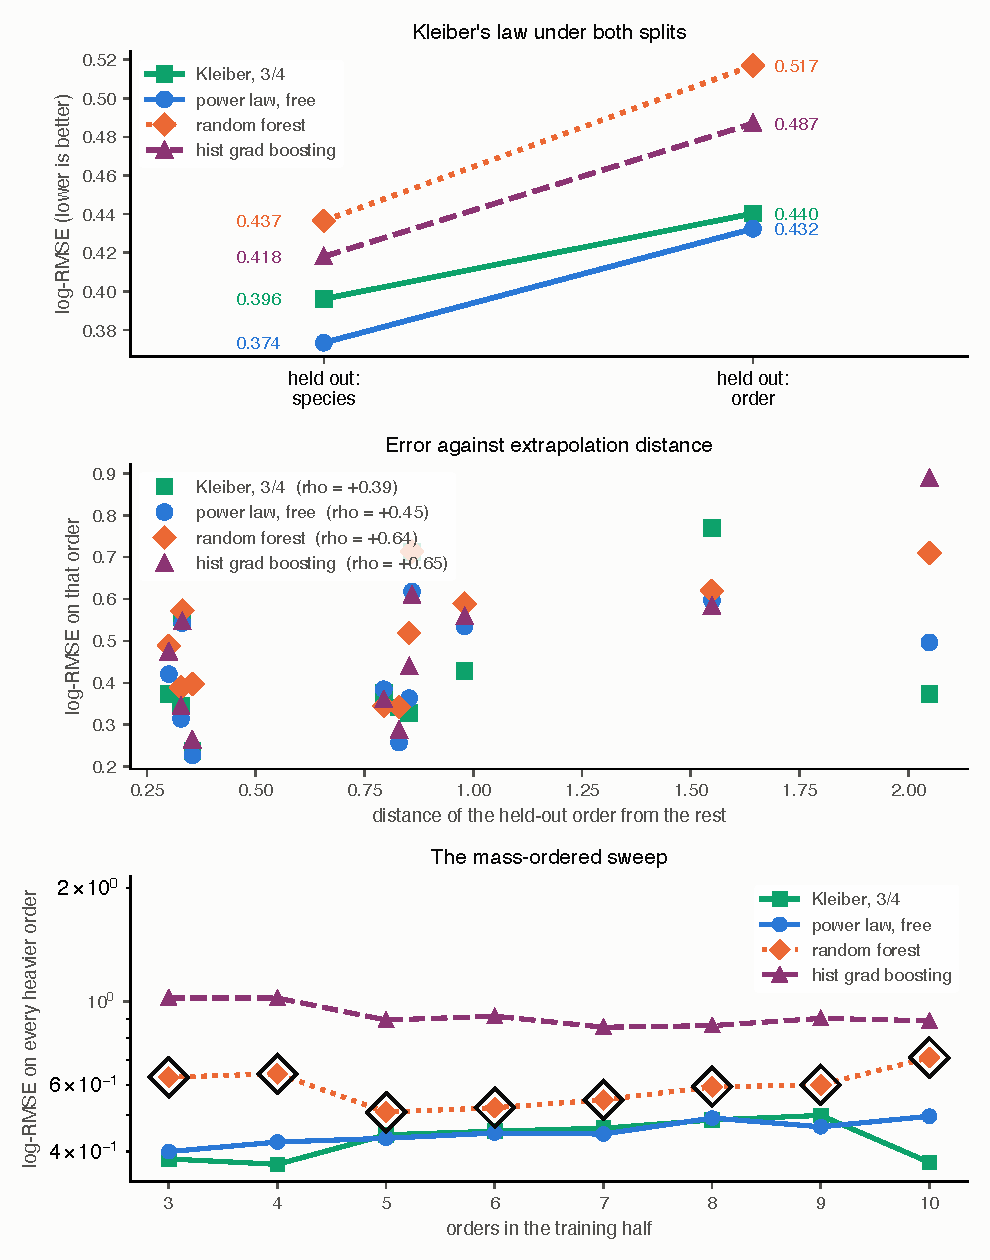
\includegraphics[width=\linewidth]{allometry}
\caption{\textbf{Kleiber's law under the same three splits.} Top: no inversion,
because the trees lose under both splits and so have no interpolation margin to
give up. Middle: error against extrapolation distance, rising for the flexible
models as it does on the ITPA H-mode database. Bottom: the mass-ordered sweep, with the circled
points marking cuts where the random forest is held inside its training
range.}
\label{fig:allometry}
\end{figure}

\section{The reversal's precondition, measured directly}
\label{sec:ladder}

Sec.~\ref{sec:allometry} leaves an asymmetry. The extrapolation failure
reproduced in full on Kleiber's law; the ranking inversion did not, and the
explanation offered there was a conjecture: with a single predictor a tree has
little to exploit, never wins the interpolation split, and so has no advantage
to lose. Two datasets cannot test that, because HDB5 and the mammalian
compilation differ in feature count and also in science, group structure, sample
size and noise.

A third dataset can probe that with a nested predictor ladder on the same rows
and splits. The Biomass And Allometry Database~\cite{baad} records, for
individual plants, a nested set of measurements: basal diameter, height, leaf
area and leaf mass. Taking the rows complete in all four gives 3599 plants
across 53 species, 33 of them with the 30 individuals required to hold a
species out, spanning 36x in diameter across species medians and over seven
orders of magnitude in mass. It is released CC0 and pinned by SHA-256 as the
other deposits are. Species plays the part of tokamak, diameter the part of
machine size, and the branching-network prediction that mass scales as diameter
to the 8/3~\cite{wbe} the part of IPB98(y,2): an exponent derived from theory
rather than fitted, which refits here to 2.512 and costs 0.5641 against 0.5780
in sample when held.

Each rung of the ladder is a prefix of the next and all four are scored on the
same rows. The rows, the splits and the model specifications are held fixed;
each rung adds one named predictor to the nested feature set. Predictor count is
therefore what is varied, but not the only thing that changes with it, since
each added column carries its own biological information. The split structure matters and is easy to get wrong:
grouped cross-validation by discharge keeps every machine on both sides, so its
analogue keeps every species on both sides. Grouping the cross-validation by
species instead would be a second leave-one-group-out, and against it no
reversal can appear at any dimension.

\begin{table}[t]
\centering
\small
\caption{The best tree ensemble's margin over the log-linear power law, on 3599
plants held fixed across the four rungs. Positive favours the trees. The
interpolation column crosses zero; the extrapolation column does not, and grows
slightly against them.}
\begin{tabular}{lrrr}
\toprule
predictors & interp.\ gain & held-out gain & reversal \\
\midrule
diameter & $-1.7\%$ & $-10.5\%$ & no \\
$+$ height & $-0.6\%$ & $-10.8\%$ & no \\
$+$ leaf area & $+1.8\%$ & $-13.1\%$ & yes \\
$+$ leaf mass & $+6.8\%$ & $-13.4\%$ & yes \\
\bottomrule
\end{tabular}
\label{tab:ladder}
\end{table}

Table~\ref{tab:ladder} and Figure~\ref{fig:ladder} separate two statements that
had been travelling as one.
The interpolation margin rises monotonically and crosses zero between two and
three predictors. The extrapolation margin does not shrink as the trees improve;
it widens, and the power law wins the held-out species at 4 of 4 rungs. The
inversion therefore appears at 3 predictors and every rung above, which is
exactly where the interpolation margin turns positive. What the ladder shows is
that the inversion tracks the interpolation margin, not that three is a
threshold: each new column adds real biological information as well as a
dimension, and leaf mass in particular is closely related to the target, so the
rungs differ in more than their count.

\begin{figure}[!htbp]
\centering
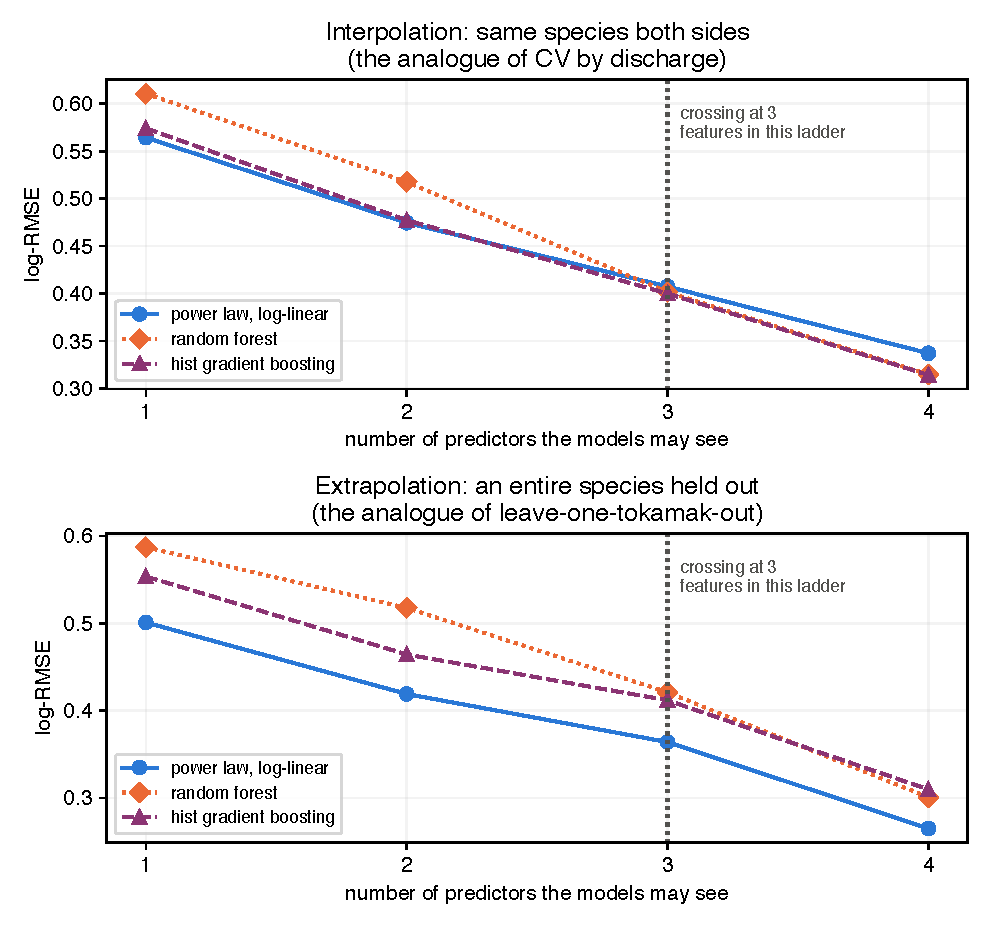
\includegraphics[width=\linewidth]{tree_allometry}
\caption{\textbf{The reversal's precondition, on 3599 plants held fixed.} Top:
the interpolation split, where every species appears on both sides. Bottom: an
entire species held out. The rows, splits and model specifications are held
fixed; each rung adds one named predictor to the nested set. The top curves
cross; the bottom ones do not.}
\label{fig:ladder}
\end{figure}

So the extrapolation failure reproduces in all three datasets tested here, at
every predictor count tested. In this ladder the extrapolation disadvantage
persists at every rung, while the ranking inversion appears only once the
flexible model gains an interpolation advantage. The inversion is therefore not
necessary for the extrapolation failure, and is better read as a visible symptom
of it than as the thing itself. At the one- and two-predictor rungs the same
qualitative extrapolation hazard is present without an interpolation advantage
whose loss would signal it.



\section{The three-kernel Gaussian-process ladder}

The main text states the ordering across three Gaussian-process kernels and
builds its mean-function ablation on it. The ladder itself is here: the same log
features, the same optimiser and the same rows, differing only in which kernel
terms exist. Table~\ref{tab:supgp} gives the scores, and
Figure~\ref{fig:gp} shows them beside the spread of each rung's predictions,
which is where a model that has reverted to a constant becomes visible as such.

\paragraph{Specification.} The three kernels are a squared-exponential with a
single isotropic length scale shared across the standardised log features, a
dot-product kernel, and their sum, each with an additive \texttt{WhiteKernel}
for observation noise. The prior mean is constant and \texttt{normalize\_y} is
on, which puts it at the training mean of $\log\tau$: this is what makes
``reverts to the prior'' and ``returns the average training target'' the same
statement, and the parallel with a tree ensemble exact. Hyperparameters are
fitted by maximising the log marginal likelihood on a seeded subsample of 1000
training rows; the kernel is then frozen and the exact GP is conditioned on
\emph{every} training row of that fold. No held-out row enters either stage.
Every rung starts from the same initialisation for every term it has, so the
three fits differ only in which terms exist. Hand-chosen hyperparameters are not
adequate here, since a length scale an order of magnitude from the one the data
supports makes the third rung look like a failure. Intervals quoted for these
models are equal-tailed posterior intervals on $\log\tau$ that include the
fitted observation-noise term, exponentiated to $\tau$. The kernel equations,
initialisations and bounds are in Sec.~\ref{supp:spec}.

\begin{table}[t]
\centering
\small
\caption{log-RMSE under the three splits, and the rank correlation of per-label
error against extrapolation distance. The intended difference across the first
three rows is whether the kernel admits a trend that continues at long range;
adding the linear term also enlarges the function class. The three span a factor
of ten at the ITER-size-matched cut. IPB98(y,2) is a historical reference
fitted to the DB2.8 predecessor of this database~\cite{hdb5} and is not
refitted within these folds.}
\begin{tabular}{lrrrr}
\toprule
model & CV & held-out & ITER cut & $\rho$ \\
\midrule
GP, linear $+$ RBF & \textbf{0.112} & 0.218 & \textbf{0.191} & $-0.01$ \\
GP, RBF only & 0.142 & 0.541 & 1.948 & $+0.65$ \\
GP, linear only & 0.181 & 0.214 & 0.278 & $-0.06$ \\
random forest & 0.128 & 0.465 & 0.938 & $+0.85$ \\
IPB98(y,2), historical ref.\ & 0.199 & 0.188 & 0.194 & $-0.49$ \\
mean baseline & 0.869 & 0.994 & 1.459 & $+0.56$ \\
\bottomrule
\end{tabular}
\label{tab:supgp}
\end{table}

\begin{figure}[!htbp]
\centering
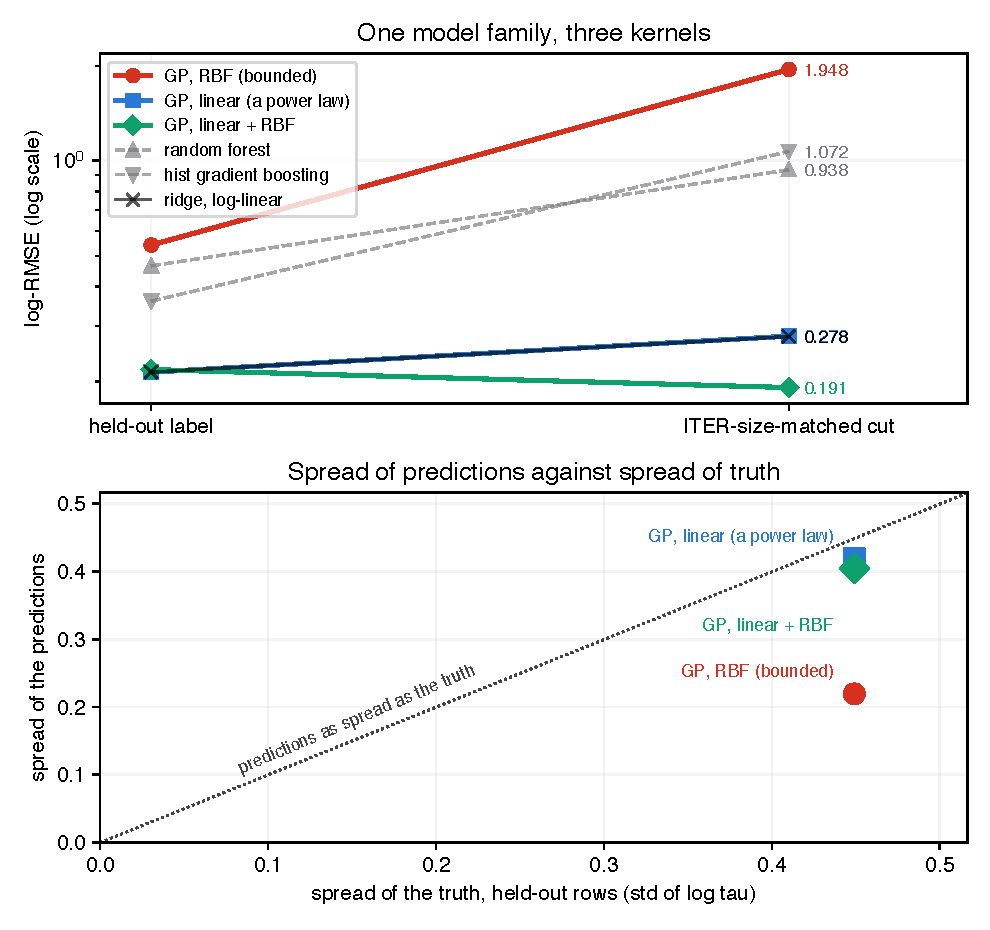
\includegraphics[width=\linewidth]{gp}
\caption{\textbf{One model family, three kernels.} Gaussian processes with a
radial-basis-function (RBF) kernel, a linear (dot-product) kernel, and their
sum. Top: log-RMSE on a held-out label and at the ITER-size-matched cut. The
kernels differ in whether they permit a trend that continues at long range;
adding the linear component also enlarges the function class. Bottom: spread of
the predictions against spread of the truth on the held-out rows. A model whose
posterior has reverted to its prior mean predicts nearly the same value
everywhere, so its spread sits near zero however good its in-range fit was: the
same failure a tree ensemble shows when it cannot exceed its largest training
target, reached by a different route.}
\label{fig:gp}
\end{figure}

The control behaves as intended: the linear-kernel process and ridge agree to $0.0000$ under
cross-validation and on a held-out label, and to $0.0007$ at the ITER-size-matched
cut, which is what licenses reading the other two rows as consequences of the
kernel. The bounded rung then fails exactly as a tree does. It beats the power
law under cross-validation and scores 1.948 at the ITER-size-matched cut, worse than
predicting a constant, with error tracking distance at $\rho = +0.65$. The
mechanism is the one in the main text: a random forest cannot exceed
the largest training target, and an RBF process reverts to its prior mean. Both are
structural long-range behaviours rather than tuning shortfalls, and on the
held-out rows this one's
predictions carry half the spread of the truth.

Adding a dot-product term to that same kernel keeps the nonlinear RBF component
it already had and supplies an unbounded linear trend alongside it. Flexibility
is retained rather than held exactly fixed, since a linear kernel enlarges the
function class as well as changing the asymptote; what the comparison isolates
is the availability of a continuing trend. It gives the best
cross-validated score in this work, 0.112 against the random forest's 0.128; it
scores 0.191 at the ITER-size-matched cut, better than the analytic law, which
is a historical reference rather than a fold-fitted competitor, and second only
to the constrained fit of
the main text at 0.183; and its error is flat against distance at
$\rho = -0.01$.


\section{Full model, kernel and split specification}
\label{supp:spec}

This section carries the settings the main text points at. ``Library
defaults'' is not a specification, and a default may differ in a later
release, so the consequential settings are written out rather than
referenced. Library versions are pinned in the repository's
\texttt{constraints.txt} and named in the main text.

\subsection{The models of the headline comparison}

The power law is \texttt{StandardScaler} followed by \texttt{Ridge} with
$\alpha=1$ and the SVD solver, chosen before any held-out score was computed and
never varied. The random forest is \texttt{RandomForestRegressor} with 300 trees,
\texttt{criterion="squared\_error"}, unlimited depth,
\texttt{min\_samples\_split}~$=2$, \texttt{min\_samples\_leaf}~$=1$,
\texttt{max\_features}~$=1.0$ and bootstrap resampling. That last setting means
every split considers all nine features rather than a random subset, so this is
bagged CART with bootstrap resampling and not the feature-subsampled forest
of~\cite{breiman}; it is scikit-learn's regression default, it is a choice
rather than an oversight, and the nested search of the main text moves off it in
13 of 19 folds. The gradient booster is
\texttt{HistGradientBoostingRegressor} with squared-error loss, learning rate
0.1, at most 100 boosting iterations, 31 leaves, no depth limit,
\texttt{min\_samples\_leaf}~$=20$, no $L_2$ penalty and 255 bins. Its
\texttt{early\_stopping="auto"} resolves to \emph{off} at every sample size
here, since that setting enables early stopping only above 10\,000 rows and no
training fold reaches that. The polynomial controls are
\texttt{PolynomialFeatures} of degree 2 and 3 without a bias column, then the
same scaler and ridge. Neither tree ensemble is standardised, which is
immaterial to both.

\subsection{The Gaussian-process kernels}

The three kernels are
\begin{align}
k_{\text{RBF}}(x,x') &= \sigma_r^{2}\,
  \exp\!\left(-\tfrac{1}{2}\lVert x-x'\rVert^{2}/\ell^{2}\right) + \sigma_n^{2}\delta_{xx'},
  \nonumber\\
k_{\text{lin}}(x,x') &= \sigma_l^{2}\,(x^{\!\top}\!x' + \sigma_0^{2})
  + \sigma_n^{2}\delta_{xx'},
  \nonumber\\
k_{\text{lin+RBF}}(x,x') &= k_{\text{lin}} + k_{\text{RBF}} - \sigma_n^{2}\delta_{xx'},
\end{align}
with a single isotropic length scale $\ell$ shared across the standardised log
features, so the RBF component is isotropic rather than
automatic-relevance-determining. Features are standardised inside the pipeline,
so each fold's scaler is fitted on that fold's training rows alone and $\ell$ is
in those units. The prior mean is constant and \texttt{normalize\_y} is on, which
puts it at the training mean of $\log\tau$: this is what makes ``reverts to the
prior'' and ``returns the average training target'' the same statement, and the
parallel with a tree ensemble exact. Observation noise enters as an additive
\texttt{WhiteKernel} rather than through a fixed jitter. Hyperparameters are
fitted by maximising the log marginal likelihood with scikit-learn's default
L-BFGS-B optimiser, \texttt{n\_restarts\_optimizer}~$=0$, from the shared
initialisation $\sigma_l^{2}=1$, $\sigma_0=1$, $\sigma_r^{2}=0.5$, $\ell=1$,
$\sigma_n^{2}=0.05$, under the bounds $\sigma_l^{2},\sigma_0 \in [10^{-3},
10^{3}]$, $\sigma_r^{2}\in[10^{-3},10^{3}]$, $\ell\in[10^{-2},10^{3}]$ and
$\sigma_n^{2}\in[10^{-6},1]$. Every rung starts from the same values for every
term it has, so the three fits differ only in which terms exist. The
optimisation runs on a subsample of exactly 1000 training rows drawn without
replacement by \texttt{numpy.random.default\_rng(42)}, or on the whole fold when
it holds fewer; the kernel is then frozen and the exact GP is conditioned on
\emph{every} training row of that fold, which is one Cholesky factorisation. No
held-out row enters either stage. Hand-chosen hyperparameters are not adequate
here, since a length scale an order of magnitude from the one the data supports
makes the third rung look like a failure. Intervals quoted for these models are
equal-tailed posterior intervals on $\log\tau$ that include the fitted
observation-noise term, exponentiated to $\tau$.

\section{Per-label scores and the eligibility-threshold sweep}
\label{supp:permachine}

Both results are stated in prose in the main text. The tables are here for a
reader who wants the per-unit numbers behind them:
Table~\ref{tab:permachine} gives the leave-one-label-out scores the distance
correlation is computed over, Table~\ref{tab:threshold} the sweep of the row
threshold that decides which labels are scored at all, and
Figure~\ref{fig:size} the full size-ordered sweep whose matched cut the main
text reports.

\begin{table}[t]
\centering
\small
\caption{Per-label log-RMSE under leave-one-label-out, ordered by Mahalanobis
distance of the held-out label's mean log-feature vector from the training
mean (computed through the pseudo-inverse, since that covariance is singular:
the design matrix is rank deficient by two, as the main text shows). The trees degrade with distance; the power law does not.}
\label{tab:permachine}
\begin{tabular}{lrrrrrr}
\toprule
Held out & rows & dist. & IPB98 & ridge & hist GB & forest \\
\midrule
D3D & 388 & 1.1 & 0.252 & 0.251 & 0.246 & 0.406 \\
AUG & 1377 & 1.2 & 0.197 & 0.216 & 0.281 & 0.279 \\
AUGW & 767 & 1.6 & 0.218 & 0.207 & 0.212 & 0.219 \\
JETILW & 866 & 1.7 & 0.257 & 0.216 & 0.244 & 0.318 \\
JET & 1762 & 2.2 & 0.148 & 0.198 & 0.487 & 0.478 \\
JT60U & 100 & 2.5 & 0.275 & 0.285 & 0.307 & 0.291 \\
PDX & 97 & 4.0 & 0.227 & 0.233 & 0.323 & 0.407 \\
ASDEX & 431 & 5.2 & 0.131 & 0.194 & 0.207 & 0.507 \\
MAST & 39 & 5.4 & 0.136 & 0.154 & 0.317 & 0.581 \\
JFT2M & 69 & 5.4 & 0.095 & 0.094 & 0.234 & 0.450 \\
CMOD & 45 & 6.9 & 0.119 & 0.173 & 0.569 & 0.521 \\
NSTX & 185 & 7.8 & 0.222 & 0.289 & 0.686 & 0.857 \\
PBXM & 59 & 10.2 & 0.172 & 0.274 & 0.559 & 0.727 \\
\bottomrule
\end{tabular}
\end{table}

\begin{table}[!htbp]
\centering
\small
\caption{Leave-one-label-out at four eligibility thresholds. Only the set of
labels scored changes across rows; the training folds and the models are
identical throughout. The 30-row threshold is the one reported elsewhere in
this paper. $p$ is the exact two-sided sign test on the win count.}
\label{tab:threshold}
\begin{tabular}{rrrrrr}
\toprule
min.\ rows & labels scored & power law & forest & forest worse on & $p$ \\
\midrule
10 & 15 & 0.262 & 0.473 & 14 of 15 & $9.8\times10^{-4}$ \\
20 & 13 & 0.214 & 0.465 & 13 of 13 & $2.4\times10^{-4}$ \\
30 & 13 & 0.214 & 0.465 & 13 of 13 & $2.4\times10^{-4}$ \\
50 & 11 & 0.223 & 0.449 & 11 of 11 & $9.8\times10^{-4}$ \\
\bottomrule
\end{tabular}
\end{table}

\begin{figure}[!htbp]
\centering
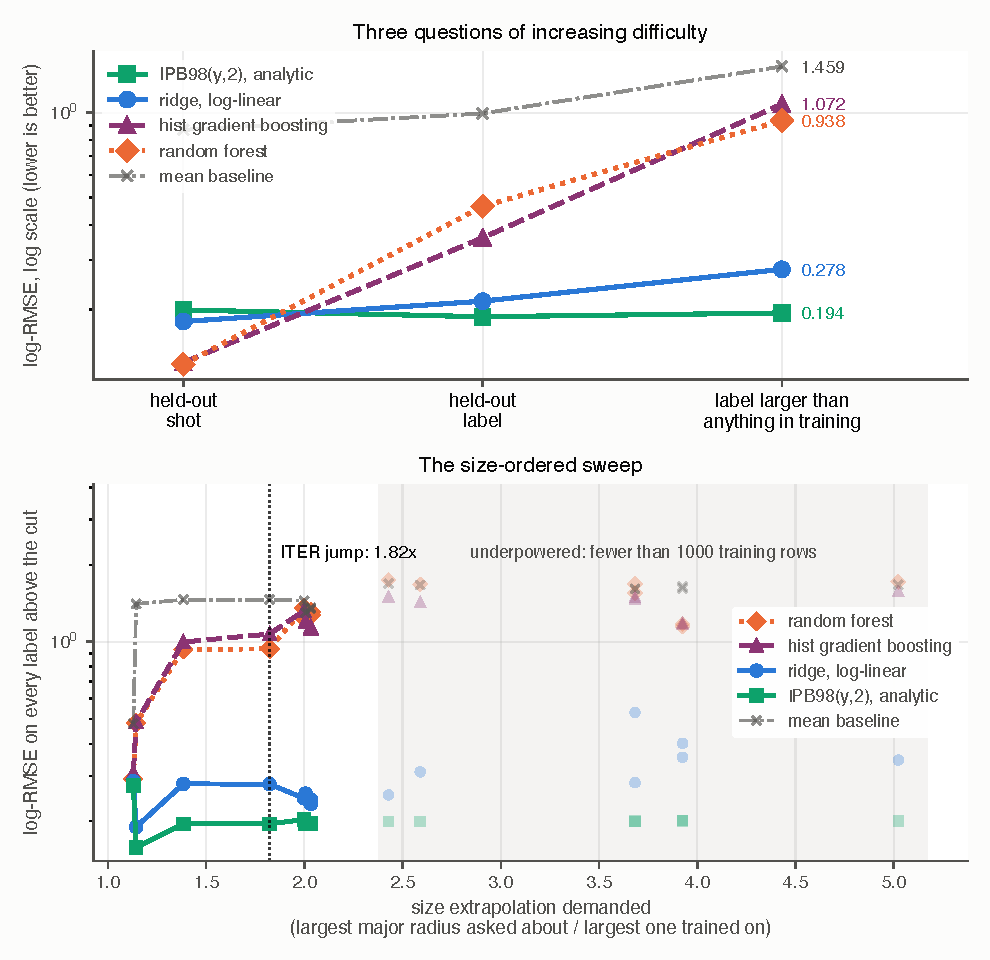
\includegraphics[width=\linewidth]{size_extrapolation}
\caption{\textbf{Size-ordered extrapolation.} Top: the escalation across three
splits of increasing difficulty, where the tree ensembles collapse toward the
mean baseline. Bottom: the sweep across every cut, with underpowered cuts drawn
faint and excluded from claims. The power law holds across the sweep and the
trees do not recover.}
\label{fig:size}
\end{figure}

\section{A power law with a bounded correction}
\label{supp:hybrid}

The diagnosis in Sec.~4.1 of the main text suggests a specific repair. Fit the
power law, learn a correction on its log residuals, and damp it by $\lambda$:
\begin{equation}
\log\tau = \underbrace{f_{\text{ridge}}(x)}_{\text{unbounded, log-linear}}
         + \lambda\,\underbrace{g(x)}_{\text{correction on residuals}} .
\end{equation}
At $\lambda=0$ this is exactly the ridge row of Table~1 of the main text.
Anchoring a learned correction on a frozen power law is also the design used in
concurrent work on this database~\cite{wang}, and this section makes no claim on
that idea. What is varied is the one property the diagnosis points at, the
long-range behaviour of the correction: one corrector is a degree-2 log
polynomial, which is unbounded, and the other is depth-2 boosted trees, which
never left the residual range they were trained on here. The two families differ
in more than that, and the controlled version of the comparison is
Sec.~12.1 of the main text. The damping factor is swept over nine values from 0
to 1, both correctors carry deliberately strong penalties so that $\lambda$
rather than their own regularisation does the damping, neither corrector's
hyperparameters are tuned, and the whole estimator is refitted from scratch
inside every training fold; the exact specification is in
\texttt{analysis\_hybrid.py} in the archived code.

Across the ITER-size-matched cut the two correctors go opposite ways. Both start
at 0.278; the polynomial correction climbs to 0.356 and the bounded correction
falls monotonically to \textbf{0.206}, better than plain ridge on all three
held-out labels and by the widest margin on the most distant of them, JT-60U
(0.440 to 0.281).

The mechanism is measurable. Fitted on the 14 small labels, the base power law
is \emph{biased} on the held-out ones, at a mean log residual of $-0.218$, so it
over-predicts by about 20\%, while its scatter (0.172) is no worse than
in-sample (0.187). The tree correction never leaves its training range on any
held-out row, and inside that bound it points the right way and is largest where
the bias is largest. The same bounded range that makes these ensembles useless
as predictors of $\tau$ on a larger machine limits how much extrapolation error
the correction can contribute, because the quantity they are bounded on is no
longer a target that grows with machine size but a residual centred on zero.
Bounded is not the same as right: a correction confined to that range can still
point the wrong way, and what is measured here is that on these rows it does
not.

Two limits qualify every later summary of this section. Cross-validation selects
$\lambda=1$ in both families while the rung best on a held-out label is
$\lambda=0$, so a practitioner tuning on the split they would ordinarily use
does not arrive at the rung that transfers. And scored at every rung of the size
sweep rather than only the matched one, the bounded hybrid wins at 5 of 8
well-powered cuts, not all, with no rule over those eight points separating wins
from losses. The claim that survives is narrow: at the cut matching the jump to
ITER, the bounded hybrid equals the power law at $\lambda=0$, where it is that
model, and beats it at all eight non-zero damping settings swept there, with the
mechanism measurable.

\section{The estimator this split design is usually paired with}
\label{supp:mixed}

Every
comparison above sets a pooled global fit against ensembles. The
clustered-validation literature cited here for the split
design~\cite{roberts} pairs that design with a third kind of estimator: a mixed
model carrying a random intercept per device, from which a device never seen is
predicted by the population-level fixed effects alone. It is neither a power law
nor a tree, it is the fit matched to the deployment question, and it is scored
here rather than conceded.

Write $\log\tau_{ij} = x_{ij}^{\prime}\beta + u_i + \varepsilon_{ij}$ with
$u_i\sim N(0,\sigma_u^2)$ over devices, fit the variance components by
restricted maximum likelihood, and predict a held-out device as
$x^{\prime}\beta$. One quantity separates this from the pooled fit, the ratio
$\lambda = \sigma_u^2/\sigma^2$. At $\lambda=0$ the estimator \emph{is} the
pooled power law, and it reproduces the ridge column of
Table~2 of the main text to three decimals by label, at 0.214, and to two by
device, at 0.212 against 0.211: the closed-form least squares this estimator
reduces to and the ridge spelling of the same fit part company in the fourth
decimal, which is the size of the penalty and not of a disagreement. As $\lambda$ grows the intercept absorbs more of the between-device
variation, which leaves $\beta$ identified increasingly by variation within a
device; major radius and aspect ratio are constant within a device by
construction, and elongation and isotopic mass nearly so, which is exactly the
identification a projection to a new machine cannot use.

The measurement follows that algebra. REML puts $\lambda$ between 1.4 and 8.1
across the 13 label folds and between 2.0 and 143 across the 11 device folds,
which is the spread eleven groups buy, and the held-out score tracks it: 0.264
per label against the power law's 0.214, and \textbf{0.829} per device against
0.212, worse on 10 of the 11 devices. Because that optimum is unstable, $\lambda$
is swept as well as fitted, which bounds what any rule for choosing it could
deliver. Over devices the score rises monotonically with $\lambda$ and is best
at $\lambda=0$, where the estimator is the pooled fit; over labels the best rung
is $\lambda=0.01$ at 0.2127 against 0.2141, a gain of 0.0014. The
deployment-matched estimator therefore does not beat a pooled power law on an
unseen device even when its one free quantity is chosen against the score it is
being judged on. Across the ITER-size-matched cut it does help, at 0.255 against
the pooled fit's 0.279, which is the least-squares spelling of the ridge row's
0.278, and it stays well above the constrained fit of
Sec.~8 of the main text at 0.183 and the analytic law's 0.194. What has been ruled out is
narrower than the class: this is a single random intercept and no random slopes,
so a device-level \emph{level} shift is what fails to be the missing structure,
and a richer hierarchical specification is untested. Eleven devices is also few
enough that the variance component is poorly determined, which is why the sweep
rather than the fit carries the conclusion. The specification and the full sweep
are in \texttt{analysis\_mixed\_model.py} and
\texttt{results/mixed\_model.json}.

The win counts support an exact test, under a null that is worth naming
precisely. Call it the independent-unit-sign null: each unit, label or device
as the case may be, is assigned to either model independently with equal
probability. Under it, losing 13 of 13 has
two-sided $p=2.4\times10^{-4}$ and losing 11 of 11 has $p=9.8\times10^{-4}$. The
device-collapsed count is the one to quote, since the 13 database labels are not
13 independent devices, and the same non-independence is a reason to prefer
these counts to the 13-label bootstrap.

That null is an idealisation, and Sec.~2 of the main text says in what way: any two
of these fits share all but two of their training machines, so the outcomes are
correlated through the training set even where the held-out devices are
distinct. The descriptive statement carries the claim on its own. The forest is
worse on every physical device scored, and the paired interval on the per-device
difference excludes zero.

\section{Four choices that do not carry the reversal}
\label{supp:choices}

\paragraph{The labels too small to score at all.} Five labels hold fewer than
30 rows (COMPASS, TCV, START, TDEV and TFTR, 43 rows between them, under 1\% of
the database) and none can carry a held-out score of its own. They are
nonetheless in every training fold, since the threshold governs scoring rather
than training, and they are among the most unusual points in the feature space,
so whether a flexible model can exploit those few rows is a fair question to ask
of the ranking.

Dropping them from training as well answers it. Every fitted model gets slightly
worse without them, by 0.012 for the power law, 0.027 for the gradient booster
and 0.007 for the random forest, and the ordering over the 13 held-out labels is
unchanged: power law 0.214 to 0.226, gradient booster 0.359 to 0.387, random
forest 0.465 to 0.472. The 43 rows help the tree ensembles slightly, as one
would expect of rows in a sparse region, and nowhere near enough to recover the
inversion. The analytic reference is unaffected, since it fits nothing.

\paragraph{Where the row threshold is set.} The 13-of-13 count is reported at a
30-row eligibility threshold, which is a choice, so it is swept.
Sec.~\ref{supp:permachine} scores leave-one-label-out at 10, 20,
30 and 50 rows. Only which labels are \emph{scored} changes: every label stays in every
training fold at every threshold, so the models being compared do not change.
The power law wins every scored label at 20, 30 and 50 rows, and 14 of 15 at 10
rows, where the exception is TCV. TCV carries 11 rows, which is why it sits
below the threshold in the first place, and a per-label log-RMSE over 11 rows
is not a quantity this paper would report on its own. The mean gap moves between
$+0.211$ and $+0.251$ across the four thresholds and the sign test stays below
$10^{-3}$ throughout, so the headline does not depend on where the line is
drawn.

\paragraph{One partition, or any partition.} The cross-validation column comes
from a single deterministic \texttt{GroupKFold} assignment of discharges to five
folds. Since this paper is about validation protocol, whether the 29\% margin is
peculiar to that one partition is a fair question. Repeating the comparison over
ten shuffled assignments of the same discharges into the same number of folds
gives a mean forest advantage of 27.8\% over the power law, ranging from 27.0\%
to 28.5\%, with the forest ahead in all ten. The deterministic partition's 29.5\%
sits just above that range, so the reported margin is if anything mildly
favourable to the forest, and the interpolation win it later gives up is a
property of the comparison rather than of one fold assignment.

One ordering inside that sweep is not resolved and the main text says so. The
two ensembles are separated by 0.002 in Table~1 of the main text, and across
these ten partitions the forest is ahead of the gradient booster in only 2 of
10, and the deterministic partition is one of the two. What every partition
agrees on is the power law's position, last of the three under cross-validation
and first under leave-one-out, which is the comparison the paper's argument
rests on. Which of the two ensembles is nominally best under cross-validation is
a coin the partition tosses, and no claim here turns on it.

\paragraph{Tuning the flexible models.} Every score above uses the
prespecified, untuned settings of Sec.~2 of the main text, which leaves open
whether the ensembles lost only because they were not hyperparameter-tuned. That is tested by giving both a grid search
nested inside each training fold: three grouped inner folds by discharge over
the training rows only, so the held-out discharge fold, label or size cut
never takes part in choosing a hyperparameter. The forest searched
\texttt{max\_features} over $\{1.0, 0.5, \text{sqrt}\}$ and
\texttt{min\_samples\_leaf} over $\{1, 5\}$, the booster
\texttt{learning\_rate} over $\{0.05, 0.1\}$ and \texttt{max\_leaf\_nodes} over
$\{15, 31\}$.

The search does real work on the forest and changes nothing about the
conclusion. It moved away from the baseline \texttt{max\_features}~$=1.0$,
\texttt{min\_samples\_leaf}~$=1$ setting in 13 of the 19 folds, and it helps where
the paper says a flexible model should help: cross-validation improves from
0.128 to 0.126 and the leave-one-label-out mean from 0.465 to 0.403. At the
ITER-size-matched cut it makes the forest \emph{worse}, 0.938 to 1.121, against the
power law's 0.278. The booster's search returned scikit-learn's defaults in all
19 folds, so its numbers are unchanged.

The inner folds above group by discharge, which is how a practitioner would
ordinarily tune. Grouping them by whole machine instead matches the way the
model is deployed, and it helps both models: the forest falls to 0.376 and the
booster to 0.350. Both remain well above the power law's 0.214, so the reversal
survives either selection procedure.

Tuning therefore widens the interpolation margin that later inverts and does
not repair the extrapolation failure, which is what the training-target bound
predicts: no setting of these hyperparameters moves a ceiling that comes from
averaging training targets.

\paragraph{Two conventions this paper does not follow.} Neither the population
nor the weighting used above matches how the ITPA scalings were produced, and
both are choices rather than findings, so both are measured.

IPB98(y,2) was fitted on a selection that excluded spherical tokamaks; this
database does not, and MAST and NSTX are two of the 13 scored labels and two of
the four most distant. The main text controls for this only at the
ITER-size-matched cut. Dropping every label whose median inverse aspect ratio exceeds 0.5, which
removes MAST, NSTX and START and 232 rows, from training and scoring alike,
leaves the reversal intact: the forest is worse than the power law on all 11
remaining labels, mean gap $+0.182$, exact $p=9.8\times10^{-4}$, at 0.395
against the power law's 0.212. The inversion is not an artefact of including
the spherical devices.

The weighting arm is the one that qualifies the headline. Every fit above
weights rows equally, so JET and ASDEX Upgrade, which supply 77\% of them, set
most of what each model learns. Refitting every model with each label weighted
equally hurts the power law more than the forest, 0.214 to 0.259 against 0.465
to 0.447, and the win count falls from 13 of 13 to \textbf{12 of 13}
($p=3.4\times10^{-3}$, mean gap $+0.188$). The label that changes hands is
AUG-W, whose unweighted margin was the second narrowest of the thirteen at
$+0.012$, behind JT-60U's $+0.006$ which does not change hands, and
which moves to $-0.067$. The direction and its significance survive the
reweighting; unanimity does not, and the 13 of 13 quoted throughout is the
unweighted count.

\section{The same distance in dimensionless coordinates}
\label{supp:dimensionless}

 Organising anything
in this field by engineering variables invites one objection, and it is the
objection Hall \emph{et al.}~\cite{hall26} have raised in a conference presentation: the weak size dependence in
this database may come from a subset localised in \emph{dimensionless} space
rather than from size, in which case a distance in engineering space measures a
shadow of the thing that matters. That is checkable here rather than only
citable. The Connor--Taylor constraints of Sec.~8 of the main text are
derived in code from the scalings of $\rho^{*}$, $\beta$ and $\nu^{*}$, so the
group definitions are already written down, and the stored energy joined across
in Sec.~4.2 of the main text supplies the temperature they need. Placing every
row by
\begin{equation}
\rho^{*}\sim T^{1/2}B^{-1}L^{-1},\qquad
\beta\sim nTB^{-2},\qquad
\nu^{*}\sim nLT^{-2},
\label{eq:supp-groups-empirical}
\end{equation}
with $T\sim W_{\mathrm{th}}/(nV)$ and $V\sim Ra^{2}\kappa$, and repeating the
distance construction above on those three coordinates instead of the nine,
gives a second ranking of the 13 labels. Multiplicative constants are dropped
throughout and cannot matter, since every quantity here is a difference of mean
log-vectors.

The two rankings agree at $\rho=+0.78$, and the diagnosis does not depend on
which is used. On the 6214 rows a dimensionless placement is possible for, the
forest's per-label error tracks dimensionless distance at $\rho=+0.77$ against
$+0.79$ for engineering distance, the booster at $+0.35$ against $+0.51$, and
the power law is flat against both, $-0.04$ and $-0.06$. The headline $+0.85$ is
the engineering figure on all 6228 rows; dropping the 14 rows with no stored
energy moves it to $+0.79$, and the coordinate change then moves it by 0.02.
The distance reading above survives translation into the coordinates the
objection is stated in.

The size cut does not fare as well, and this is where the objection lands. At
the ITER-size-matched cut the two sides are separated in dimensionless space as
well as in size: the interquartile ranges of $\log\rho^{*}$ do not overlap at
all and its median moves by 1.21 training standard deviations, $\log\nu^{*}$
overlaps by 0.26 at 0.85 standard deviations, and only $\log\beta$ stays put,
overlapping by 0.69 at 0.22. Larger machines in this database run at smaller
normalised gyroradius and lower collisionality, which is physics rather than an
artefact, and it means the cut is not a size boundary with everything else held
fixed. Every result scored across it is therefore transfer across a joint
displacement in size, $\rho^{*}$ and $\nu^{*}$, and the paper says so rather
than describing it as a size extrapolation alone. The leave-one-device-out
comparison of Sec.~4 of the main text carries no such confound, which is the
second reason it and not the cut is the claim this paper rests on.

\section{What the elongation substitution costs}
\label{supp:elongation}

ITPA20 and ITPA20-IL are specified on the separatrix elongation at the geometric
axis, $\kappa$, and STD5 delivers one elongation column, \texttt{KAPPAA}: the
areal elongation $\kappa_a = S/(\pi a^2)$, which is the definition IPB98(y,2)
was fitted to. Sec.~4.2 of the main text scores each law on the column it was
fitted to, taking $\kappa$ from the full DB5.2.3 revision. What that
substitution is worth is measured here rather than modelled, and the measurement
is also the argument for not modelling it.

On a parametrised boundary $\kappa/\kappa_a$ depends on the triangularity
alone, which confines the ratio to $[1.000, 1.110]$. The measured ratio has a
median of \textbf{1.083} and a maximum of \textbf{1.341}, with 16\% of rows
above that ceiling and 7\% \emph{below} unity, which no boundary of that family
produces at all. Only \textbf{2.0\%} are below it by more than
$5\times10^{-4}$; the rest is rounding on machines that ran circular.

The rows below unity are worth following, because the obvious reading of them is
that the delivered column is wrong and the obvious reading is not right here. A
boundary elongation below the areal elongation is impossible for a \emph{convex}
boundary, and of the 2.0\% that clear rounding, all but PBX-M's 59 rows sit
within 3.5\% of unity on near-circular machines, which the two columns'
precision covers. PBX-M does not: its ratio runs from 0.67 to 0.80, at a median
of \textbf{0.739}. PBX-M ran indented, bean-shaped plasmas, its boundary is not
convex, and the convexity argument does not apply to it. DB5.2.3 records that
directly: of the analysed rows, PBX-M is the only label carrying an indentation
above 0.04, at a median of \textbf{0.154}, and the 60 rows with any indentation
at all have a median $\kappa/\kappa_a$ of 0.740. The column is not defective on
those rows; the parametrised boundary is simply the wrong shape for them, which
is the same point the ratio makes everywhere else and is here checkable against
a third column.

Scoring on the delivered column rather than the measured one moves ITPA20 by up
to 0.018 and ITPA20-IL by up to 0.022, twenty to thirty times what the shape
model would predict. Where a column exists, a model of it is not evidence about
it.

\begin{thebibliography}{99}
\small\setlength{\itemsep}{0pt}\setlength{\parskip}{0pt}
\raggedright
\bibitem{hdb5} G. Verdoolaege \emph{et al.}, ``The updated ITPA global H-mode
confinement database: description and analysis,'' \emph{Nucl.\ Fusion}
\textbf{61}, 076006 (2021).
\href{https://doi.org/10.1088/1741-4326/abdb91}{doi:10.1088/1741-4326/abdb91}
\bibitem{hall26} J. Hall, P. Zhang, Y. Zhang, C. Angioni and G. Verdoolaege,
``Confinement scaling with machine size in the updated ITPA global H-mode
energy confinement database,'' poster P2.1097, \emph{52nd EPS Conf.\ on Plasma
Physics}, Edinburgh (2026). Conference presentation; not published in refereed
form at the time of writing.
\bibitem{breiman} L. Breiman, ``Random forests,'' \emph{Machine Learning}
\textbf{45}, 5 (2001).
\href{https://doi.org/10.1023/A:1010933404324}{doi:10.1023/A:1010933404324}
\bibitem{roberts} D.R. Roberts \emph{et al.}, ``Cross-validation strategies for
data with temporal, spatial, hierarchical, or phylogenetic structure,''
\emph{Ecography} \textbf{40}, 913 (2017).
\href{https://doi.org/10.1111/ecog.02881}{doi:10.1111/ecog.02881}
\bibitem{wang} Z. Wang \emph{et al.}, ``Power-law-anchored residual learning
for H-mode energy confinement time in tokamaks: interpolation and
parameter-defined extrapolation,'' arXiv:2608.20684 (2026).
\href{https://doi.org/10.48550/arXiv.2608.20684}{doi:10.48550/arXiv.2608.20684}
\bibitem{ipb98} ITER Physics Expert Group on Confinement and Transport, ITER
Physics Expert Group on Confinement Modelling and Database and ITER Physics
Basis Editors, ``Chapter 2: Plasma confinement and transport,'' \emph{Nucl.\
Fusion} \textbf{39}, 2175 (1999).
\href{https://doi.org/10.1088/0029-5515/39/12/302}{doi:10.1088/0029-5515/39/12/302}
\bibitem{doyle07} E. J. Doyle \emph{et al.}, ``Chapter 2: Plasma confinement
and transport,'' \emph{Progress in the ITER Physics Basis}, \emph{Nucl.\
Fusion} \textbf{47}, S18 (2007).
\href{https://doi.org/10.1088/0029-5515/47/6/S02}{doi:10.1088/0029-5515/47/6/S02}
\bibitem{creely} A.J. Creely \emph{et al.}, ``Overview of the SPARC tokamak,''
\emph{J.\ Plasma Phys.} \textbf{86}, 865860502 (2020).
\href{https://doi.org/10.1017/S0022377820001257}{doi:10.1017/S0022377820001257}
\bibitem{iter89p} P.N. Yushmanov \emph{et al.}, ``Scalings for tokamak energy
confinement,'' \emph{Nucl.\ Fusion} \textbf{30}, 1999 (1990). ITER89-P.
\href{https://doi.org/10.1088/0029-5515/30/10/001}{doi:10.1088/0029-5515/30/10/001}
\bibitem{jt60saplan} JT-60SA Research Unit, \emph{JT-60SA Research Plan:
Research Objectives and Strategy}, Version 5.0 (2021).
\url{https://www.jt60sa.org/wp/wp-content/uploads/2021/02/JT-60SA_Res_Plan-5.pdf}
\bibitem{jt60saop1} M. Yoshida \emph{et al.}, ``Overview of plasma operation and
control studies in the first plasma campaign of JT-60SA,'' \emph{Plasma Phys.\
Control.\ Fusion} \textbf{67}, 065010 (2025).
\href{https://doi.org/10.1088/1361-6587/add563}{doi:10.1088/1361-6587/add563}
\bibitem{jt60saop2} J. Garcia \emph{et al.}, ``Overview of first JT-60SA plasma
operation and plans in view of ITER and DEMO,'' \emph{Nucl.\ Fusion} \textbf{66},
116011 (2026).
\href{https://doi.org/10.1088/1741-4326/ae74e1}{doi:10.1088/1741-4326/ae74e1}
\bibitem{kleiber} M. Kleiber, ``Body size and metabolism,''
\emph{Hilgardia} \textbf{6}, 315 (1932).
\href{https://doi.org/10.3733/hilg.v06n11p315}{doi:10.3733/hilg.v06n11p315}
\bibitem{baad} D.S. Falster \emph{et al.}, ``BAAD: a Biomass And Allometry
Database for woody plants,'' \emph{Ecology} \textbf{96}, 1445 (2015).
Released CC0.
\href{https://doi.org/10.1890/14-1889.1}{doi:10.1890/14-1889.1}
\bibitem{wbe} G.B. West, J.H. Brown and B.J. Enquist, ``A general model for the
structure and allometry of plant vascular systems,'' \emph{Nature}
\textbf{400}, 664 (1999).
\href{https://doi.org/10.1038/23251}{doi:10.1038/23251}
\bibitem{felsenstein} J. Felsenstein, ``Phylogenies and the comparative
method,'' \emph{Am.\ Nat.} \textbf{125}, 1 (1985).
\href{https://doi.org/10.1086/284325}{doi:10.1086/284325}
\end{thebibliography}

\end{document}
